\section{Введение в ползучесть}
В механике деформируемого тела принято различать исследуемые материалы по их 
реакции на нагрузку. Когда при произвольном процессе нагружения материал сразу же после
снятия нагрузки возвращается в исходное состояние, то говорят, что имеют дело с чисто 
упругой средой. Если после разгрузки появляются остаточные деформации, которые зависят
только от величин нагрузок и порядка их приложения, но не зависят от
скоростей нагружения и времени выдержки, то такая среда носит название 
упругопластической.
В случае же, когда эти деформации существенно зависят от времени нагружения, про такие 
среды говорят, что они обладают свойствами ползучести или в более общем виде - реологическими
свойствами.

Фактически все существующие материалы при различных температурах в той или иной мере 
обладают свойствами ползучести. Однако при определенных условиях работы материалов 
деформациями ползучести по сравнению с упругими или мгновенными пластическими 
деформациями можно пренебречь. При этом существенно упрощаются определяющие соотношения. 
Поэтому свойства ползучести учитываются только тогда, когда пренебрежение ими может 
привести к существенным ошибкам в оценке деформируемости и работоспособности исследуемых 
объектов.

Из сказанного следует, что для максимального использования потенциальных ресурсов 
материала необходимо более полно изучать его свойства, переходя от чистой упругости к 
учету пластичности и далее ползучести. Но при этом более широкий учет свойств материалов 
приводит к существенному усложнению соотношении, связывающих напряжения и деформации, что 
в свою очередь ведет к резкому росту трудностей при решении конкретных задач.
Вопросы ползучести металлов и расчета элементов конструкций с учетом ползучести 
рассматриваются в специальных монографиях [\ref{rabotnov}, \ref{malinin}, \ref{kachanov}, \ref{romanov}, \ref{lokoschenko}]

Процесс ползучести можно разделить на три стадии. В первой стадии (участок 	
ОА, рис.\ref{intro_creep}) скорость деформации ползучести постепенно уменьшается. Бейли в 1929 
(Beiley R. W.) объяснял характер кривой ползучести при разных значениях 
времени t как результат взаимодействия механического упрочнения и 
термического разупрочнения. В первой стадии преобладает механическое 
упрочнение, связанное с ростом деформации ползучести.

Во второй стадии (участок АВ, рис.\ref{intro_creep}) устанавливается равновесие между механическим 
упрочнением и термическим разупрочнением, и процесс ползучести протекает с 	минимальной 
постоянной во времени скоростью, которая зависит от напряжения и 
температуры. Длительность второго участка уменьшается с увеличением напряжения, при 
больших напряжениях она может вообще отсутствовать.			
\newpage
	\begin{figure}[h!]
		\begin{minipage}[h]{0.48\linewidth}
			\center{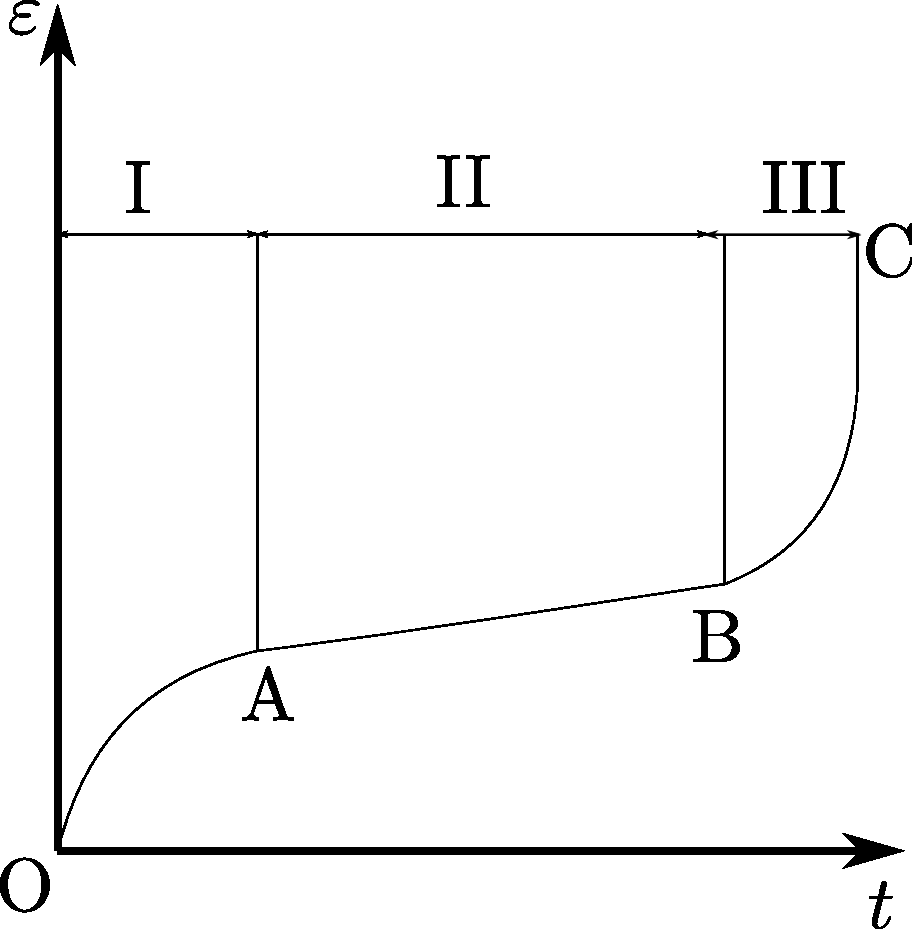
\includegraphics[width=1.0\linewidth]{images/creep.pdf}}
			\caption{Кривая ползучести}
					\label{intro_creep}
		\end{minipage}
		\hfill
		\begin{minipage}[h]{0.48\linewidth}

		В третьей стадии ползучести (участок ВС) скорость деформации непрерывно возрастает, пока 
не наступает разрушение образца (точка С).
Увеличение скорости деформации в третьей стадии объясняется или увеличением $\sigma$ 
вследствие уменьшения площади поперечного сечения образца, или образованием трещин внутри 
образца, которые развиваются в материале в течение времени под влиянием напряжений и 
температуры и ослабляют образец.
		\end{minipage}

	\end{figure}
Из испытаний следует, что увеличение напряжения и температуры интенсифицирует процесс 
ползучести, скорости деформаций ползучести при этом возрастают, продолжительность второй 
стадии и время, необходимое для разрушения, уменьшаются. При этом I стадия вообще может 
отсутствовать.

\section{Базовые модели ползучести}

\subsection{Установившаяся ползучесть}
Рассмотрим ползучесть образца при растяжении, при котором продолжительность I и III участков кривой ползучести относительно общего времени работы образца невелика, т.е. образец большую часть времени находится в состоянии установившейся ползучести. 
В этом случае для описания поведения материала естественно использовать соотношение нелинейно-вязкого течения, называющееся теорией установившейся ползучести, в котором фигурирует зависимость скорости деформаций от напряжений $\sigma$ и температуры $T$:
 \begin{equation}
 	\dot{p} = f(\sigma, T)
 \end{equation}
 
Для функции $f$ можно рассмотреть различные конкретные формы. Чаще других используются экспоненциальная зависимость:
\begin{equation} 
	\dot{p} = B_1e^{\frac{\sigma}{\gamma}},
\end{equation}
предложенная Людвиком в 1908 г., и степенная зависимость
\begin{equation} 
	\dot{p} = B\sigma^n,
\end{equation}
предложенная Бейли в 1929 г. Недостаток выражения, приводящего к ненулевой скорости ползучести $\dot{p}$ при нулевом напряжении $\sigma$ и вообще плохо описывающего свойства металлов при малых напряжениях, исправляет зависимость, предложенная А. Надаи в 1937 г.:
\begin{equation}
	\dot{p} = B\, \text{sh}(\dfrac{\sigma}{\widehat{\sigma}}).
\end{equation}
В последнее время для описания ползучести при растяжении широкое применение находит зависимость $\dot{p}$, предложенная С.А.Шестериковым и М.А.Юмашевой [\ref{shest}]:
\begin{equation}
	\dot{p} = B\left(\dfrac{\sigma-\sigma_0}{\sigma_b-\sigma}\right)^n,
\end{equation}
где $n$ и $B$~-- параметры материала, $\sigma_0$~-- минимальный уровень напряжения при котором проявляется ползучесть, $\sigma_b$~-- предел кратковременной прочности.
Полученное дробно-линейное соотношение при $\sigma_0 = 0$ одновременно описывает линейную ползучесть при $\sigma \ll \sigma_b$ и высокую степень нелинейности при $\sigma \to \sigma_b$.

